\documentclass[10pt]{beamer}
\usepackage[T1]{fontenc}
\usepackage[utf8]{inputenc}
\usepackage{lmodern}
\usepackage[english]{babel}

\usepackage{stmaryrd}
\usepackage{verbatim}
\usepackage{geometry}
\usepackage{setspace}

\usepackage{latex/agda}
\usepackage{unicode-math}
\setmathfont{XITS Math}

\setmainfont{DejaVu Serif}
\setsansfont{DejaVu Sans}
\setmonofont{DejaVu Sans Mono}


\usepackage{newunicodechar}
\newunicodechar{→}{\ensuremath{\mathnormal\to}}
\newunicodechar{ℕ}{\ensuremath{\mathbb{N}}}


\usepackage{xcolor}
\usepackage[normalem]{ulem}
\usepackage{soul}
\usepackage{amsmath}
\usepackage{amssymb}

\usepackage{multirow}
\usepackage{multicol}
\usepackage{caption}
\usepackage{bussproofs}

\usepackage{tikz-cd}
\usetikzlibrary{matrix}

\let\oldquote\quote
\let\endoldquote\endquote

\RenewDocumentEnvironment{quote}{om}
  {\oldquote}
  {\par\nobreak\smallskip
   \hfill(#2\IfValueT{#1}{~---~#1})\endoldquote
   \addvspace{\bigskipamount}}

\newcommand{\equalH}[2]{#1 = #2}
\newcommand{\comprehensionH}[3]{\{ #1 : #2 \mid #3 \}}
\newcommand{\arrowH}[2]{#1 \rightarrow #2}
\newcommand{\appH}[2]{#1 #2}
\newcommand{\equivalenceH}[2]{#1 \simeq #2}

\usetheme{Antibes}
\usecolortheme{beaver}
\useinnertheme{rounded}
\useoutertheme{infolines}

%\titlegraphic{\includegraphics[width=25mm]{gottingen1.png}}
\title{Modeling Formal Languages in Grammatical Framework}
\subtitle{On the Grammar of Proof}
\author{Warrick Macmillan}
\date{$7^{th}$ August 2021}


\begin{document}

\begin{frame}
  \titlepage
\end{frame}


% \begin{frame}
% \frametitle{Overview}
% \tableofcontents
% \end{frame}

\section{Overview}

\subsection{Introduction}
\begin{frame}
\frametitle{Table of Contents}

\begin{enumerate}

\item Explore abstract relationships between math, CS, Type Theory, and
  Linguistics
\item Practical and brief intro to MLTT and Agda
\item Grammars elaborating the abstractions above
\end{enumerate}
\end{frame}


\begin{frame}[fragile]
\frametitle{Abstraction Ladders}
\begin{columns}
\begin{column}{.5\linewidth}
\begin{tikzcd}
Strings \ar[d,"Lexical\ Analysis"] \ar[dd,bend right=+90.0, swap,"Front\ End"]
&[5m]
\\ Lexemes \ar[d,"Parsing"] &[5em]
\\ ASTs \ar[d,"Type\ Checker"] &[5m]
\\ Typed\ ASTs
  \ar[dd, bend left, "Code\ Generator"]
  \ar[dd, bend right, swap, "Interpreter"] &[5m]
\\ ...
\\ Target\ Language
\end{tikzcd}
\end{column}
\begin{column}{0.6 \linewidth}
\begin{tikzcd}
  Phonemes \arrow[d, "Morhphophonological
  \\ Anaylsis" description]
  \\ Morphemes \arrow[d, "Parse"]
  \\ \{\ Syntactic\ Representation\ \} \arrow[d, "Montague"', bend right=49]
    \arrow[d, "Ranta", bend left=49] \arrow[d, "..." description]
  \\ {\{\ STLC,\ ...\ ,\ DTT\ \}} \arrow[d, "?" description]
  \\ {\{\ Nearal Encoding\ ,\ ...\ ,\ I\ Language\ \}} \arrow[d, "?" description]
  \\ Phonemes
\end{tikzcd}
\end{column}
\end{columns}
\end{frame}

\begin{frame}[fragile]
\frametitle{Computational Trinitarianism}
\centering
\begin{tikzcd}
                                                                            &  &  & Logic \arrow[llldddd, "Denotational\ Semantics" description] \arrow[rrrdddd, "Include\ Terms" description] &  &  &                                                                                                       \\
                                                                            &  &  &                                                                                                            &  &  &                                                                                                       \\
                                                                            &  &  &                                                                                                            &  &  &                                                                                                       \\
                                                                            &  &  &                                                                                                            &  &  &                                                                                                       \\
Math \arrow[rrruuuu, "Embedded\ in\ FOL", bend left] \arrow[rrrrrr, "ITP"'] &  &  &                                                                                                            &  &  & CS \arrow[llllll, "Denotational\ Semantics", bend left] \arrow[llluuuu, "Remove\ Terms"', bend right]
\end{tikzcd}


\end{frame}


\begin{frame}[fragile]
% \frametitle{Linguistic  Interpretations}
\frametitle{Interpretation Language}
\begin{alertblock}{Observation 1.1}
  We acknowledge this is only semantic interpretations in these domains.
  One may decide on syntactic, pragmatic, or other ways in which to treat
  linguistics via these fields
\end{alertblock}
\centering
\begin{tikzcd}
     &  &  & Logic                                                                                                                     &  &  &            \\
     &  &  &                                                                                                                           &  &  &            \\
     &  &  & Linguistics \arrow[uu, "Montague\ Semantics"'] \arrow[llldd, "Distributional\ Semantics"'] \arrow[rrrdd, "TT\ Semantics"] &  &  &            \\
     &  &  &                                                                                                                           &  &  &            \\
Math &  &  &                                                                                                                           &  &  & CS\ (MLTT)
\end{tikzcd}

\end{frame}


\begin{frame}[fragile]
\frametitle{Trinitarian Linguistics }
\centering
\begin{tikzcd}
                                                &  &  & Logic \arrow[dd, "Embedding"] &  &  &                               \\
                                                &  &  &                               &  &  &                               \\
                                                &  &  & Linguistics                   &  &  &                               \\
                                                &  &  &                               &  &  &                               \\
Math \arrow[rrruu, "Language\ Of\ Mathematics"] &  &  &
&  &  & CS\ (MLTT) \arrow[llluu, "Meaning\ Explanations"]
\end{tikzcd}

\end{frame}

\begin{frame}[fragile]
\centering
\frametitle{Trinitarian Grammars}
% https://tikzcd.yichuanshen.de/#N4Igdg9gJgpgziAXAbVABwnAlgFyxMJZAZgBoAGAXVJADcBDAGwFcYkQAZCAcywGMQAX1LpMufIRTlSAFmp0mrdgFl6OABZCRIDNjwEiANlnyGLNohABhAMoAdOwAIAFMo4AVdwEotovRKIyACZTRQsQAHEAMSF5GChueCJQADMAJwgAWyRpEBwIJDIQRnoAIxhGAAUxfUlimBScEBozJUsAJXowHHoHRy5ePj7nKwBBABEAUR9hVIzsxABGGnzCmhLyqpqAy0YGppaw9k7u3qcACQgcHGGbAFU+1Q0Z7XSspCCVgsQi1vC+ZilfhMTyxQRAA
\begin{tikzcd}
                                              &  &  & Logic \arrow[dd, "Ranta\ Logic\ (CADE)"] &  &  &                                       \\
                                              &  &  &                                          &  &  &                                       \\
                                              &  &  & GF                                       &  &  &                                       \\
                                              &  &  &                                          &  &  &                                       \\
Math \arrow[rrruu, "Ranta\ Hott\ (SU\ Math)"] &  &  &                                          &  &  & CS\ (MLTT) \arrow[llluu, "cubicalTT"]
\end{tikzcd}

\end{frame}

\begin{frame}[fragile]
\frametitle{Models of  GF}
\centering
\begin{tikzcd}
     &  &  & Logic                                                                                                                                             &  &  &            \\
     &  &  &                                                                                                                                                   &  &  &            \\
     &  &  & GF \arrow[uu, "?"'] \arrow[llldd, "Theory\ of\ Operads"']
     \arrow[rrrdd, "Implementation\ of", bend left] \arrow[rrrdd, "Agda\ Embedding", bend right] &  &  &            \\
     &  &  &                                                                                                                                                   &  &  &            \\
Math &  &  &                                                                                                                                                   &  &  & CS\ (MLTT)
\end{tikzcd}

\end{frame}

\begin{frame}[fragile]
\frametitle{Remarks}
\centering
\begin{itemize}
% \begin{enumerate}
\item Trinitarian doctrine is in the ``formal" space
\item Trinitarian + Linguistics is partially formal, and very underexplored
\item Introduces many philosophical concerns, perhaps a rereading of
  Wittgenstein should take place in this context
% \end{enumerate}
\end{itemize}
\end{frame}

\section{Preliminaries and Perspectives}

\subsection{MLTT}

\begin{frame}

\begin{itemize}
  \item Frege : Formal Proof, Predicate Logic
  \item Russel : Type Theory to resolve his paradox
  \item Brouwer : Constructivism
\end{itemize}

\end{frame}

\begin{frame}

\begin{quote}{Per Martin-Löf, Padua Italy, June 1980}

Mathematical logic and the relation between logic and mathematics have been
interpreted in at least three different ways:
\newline

\\
i. mathematical logic as symbolic logic, or logic using mathematical symbolism; \\
ii. mathematical logic as foundations (or philosophy) of mathematics;\\
iii. mathematical logic as logic studied by mathematical methods, as a branch of mathematics.
\newline

\\
We shall here mainly be interested in mathematical logic in the second sense.
What we shall do is also mathematical logic in the first sense, but certainly
not in the third.
\end{quote}
\end{frame}

\begin{frame}
\frametitle{Syntactic Comparisons}

\begin{columns}

\begin{column}{0.4 \textwidth}
\begin{block}{First Order Logic}
  \begin{itemize}
    \item $\forall$
    \item $\exists$
    \item $\supset$
    \item $\wedge$
    \item $\lor$
    \item $\neg$
    \item $\top$
    \item $\bot$
    \item $=$
  \end{itemize}
\end{block}
\end{column}

\begin{column}{0.4 \textwidth}
\begin{block}{Dependent Type Theory}
  \begin{itemize}
    \item $\Pi$
    \item $\Sigma$
    \item $\to$
    \item $\times$
    \item $+$
    \item $\neg$
    \item $\top$
    \item $\bot$
    \item $\equiv$
  \end{itemize}
\end{block}
\end{column}

\end{columns}

\end{frame}

\begin{frame}
\begin{columns}

\begin{column}{0.4 \textwidth}
\begin{exampleblock}{Sets}
  \begin{itemize}
    \item $\mathbb{N}$
    \item $\mathbb{N} \times \mathbb{N}$
    \item $\mathbb{N} \to \mathbb{N}$
    \item $\{x|P(x)\}$
    \item $\emptyset$
    \item $?$
    \item $\cup$
    \item $?$
  \end{itemize}
\end{exampleblock}
\end{column}

\begin{column}{0.4 \textwidth}
\begin{block}{Types}
  \begin{itemize}
    \item $Nat$
    \item $Nat \times Nat$
    \item $Nat \to Nat$
    \item $\Sigma x : \_ . P(x)$
    \item $\bot$
    \item $\top$
    \item $?$
    \item $U_1$
  \end{itemize}
\end{block}
\end{column}
\end{columns}

\begin{columns}

\begin{column}{0.4 \textwidth}
\begin{exampleblock}{More Sets}
  \begin{itemize}
    \item $1$
    \item $(1,0)$
  \end{itemize}
\end{exampleblock}
\end{column}

\begin{column}{0.4 \textwidth}
\begin{block}{Programs}
  \begin{itemize}
    \item $suc\ zero$
    \item $(suc\ zero, zero)$
  \end{itemize}
\end{block}
\end{column}
\end{columns}

\end{frame}

\begin{frame}

\frametitle{Judgments}

\begin{columns}

\begin{column}{0.4 \textwidth}
\begin{block}{Type Theoretic Judgments}
  \begin{itemize}
  \item $T$ is a type
  \item $T$ and $T'$ are equal types
  \item $t$ is a term of type $T$
  \item $t$ and $t'$ are equal terms of type $T$
  \end{itemize}
\end{block}
\end{column}

\begin{column}{0.4 \textwidth}
\begin{block}{Mathematical Judgments}
  \begin{itemize}
  \item $P$ is a proposition
  \item $P$ is true
  \end{itemize}
\end{block}
\end{column}
\end{columns}

\\~\\
\begin{itemize}
  \item Notice that judgmental equality is uniquely type theoretic
  \item Judgments in type theory are decidable
  \item Truth (inhabitation) is not decidable
  \item More exotic judgments are available in TT, i.e. $P$ is possible.
\end{itemize}

\end{frame}


\begin{frame}

\frametitle{Important Differences}

\begin{itemize}
\item The rules of the types make explicit that they are not equivalent to those
  of classical FOL
\item An existential assertion in type theory requires data
\item Excluded middle and double negation are not admitted in MLTT
\item To be \emph{not unhappy} is clearly of a different meaning than to be \emph{happy}.
\item This makes our approach to general translation of non-constructive mathematics \emph{impossible}  (at least such that it type-checks)

\end{itemize}
\end{frame}

\begin{frame}

\begin{itemize}
\item One doesn't define logics, type systems in mathematics (e.g. metamathemeatics)
\item Encoding things like rational and real numbers in type theory are
\item already, category theorists and set theorists are at odds, (small and
  large categories), higher categories, which skeletons of categories are canonical, etc.
  incredibly difficult
\item Additionally, intensional type theory comes with two distinct notions of
  equality, judgmental/definitional/computational and propositional equality
\end{itemize}
\end{frame}

\begin{frame}

\frametitle{Example Donkey Anaphora}

Interpret the sentence ``every man who owns a donkey beats it'' in MLTT via the following judgment :

\[\Pi z : (\Sigma x : man. \; \Sigma y : donkey. \; owns(x,y)). \;
  beats(\pi_1z,\pi_1(\pi_2z))\]

We judge $\vdash man \; {:} {\rm type}$ and $\vdash donkey \; {:}
{\rm type}$. ${\rm type}$ really denotes a universe

\end{frame}

\subsection{Agda}

\begin{frame}
\frametitle{What is Agda?}

\begin{itemize}
\item Implementation of MLTT
\item Logical Framework
\item Interactive proof development environment
\item Inductive Types, Modules, Pattern Matching, & more
\end{itemize}

\end{frame}

\begin{frame}

\begin{columns}

\begin{column}{0.4 \textwidth}

\begin{block}{Mathematical Declarations}
  \begin{itemize}
    \item Theorem
    \item Proof
    \item Lemma
    \item Axiom
    \item Definition
    \item Example
  \end{itemize}
\end{block}

\end{column}

\begin{column}{0.7 \textwidth}

% \begin{code}[hide]%
\>[0]\<%
\\
\>[0]\AgdaKeyword{data}\AgdaSpace{}%
\AgdaDatatype{ℕ}\AgdaSpace{}%
\AgdaSymbol{:}\AgdaSpace{}%
\AgdaPrimitive{Set}\AgdaSpace{}%
\AgdaKeyword{where}\<%
\\
\>[0][@{}l@{\AgdaIndent{0}}]%
\>[1]\AgdaInductiveConstructor{zero}\AgdaSpace{}%
\AgdaSymbol{:}\AgdaSpace{}%
\AgdaDatatype{ℕ}\<%
\\
%
\\[\AgdaEmptyExtraSkip]%
\>[0]\AgdaKeyword{variable}\<%
\\
\>[0][@{}l@{\AgdaIndent{0}}]%
\>[2]\AgdaGeneralizable{A}\AgdaSpace{}%
\AgdaSymbol{:}\AgdaSpace{}%
\AgdaPrimitive{Set}\<%
\\
%
\>[2]\AgdaGeneralizable{D}\AgdaSpace{}%
\AgdaSymbol{:}\AgdaSpace{}%
\AgdaPrimitive{Set}\<%
\\
%
\>[2]\AgdaGeneralizable{stuff}\AgdaSpace{}%
\AgdaSymbol{:}\AgdaSpace{}%
\AgdaPrimitive{Set}\<%
\\
%
\\[\AgdaEmptyExtraSkip]%
\>[0]\AgdaFunction{definition-body}\AgdaSpace{}%
\AgdaSymbol{=}\AgdaSpace{}%
\AgdaDatatype{ℕ}\<%
\\
%
\\[\AgdaEmptyExtraSkip]%
\>[0]\AgdaFunction{T}\AgdaSpace{}%
\AgdaSymbol{=}\AgdaSpace{}%
\AgdaDatatype{ℕ}\<%
\\
\>[0]\AgdaFunction{L}\AgdaSpace{}%
\AgdaSymbol{=}\AgdaSpace{}%
\AgdaDatatype{ℕ}\<%
\\
\>[0]\AgdaFunction{E}\AgdaSpace{}%
\AgdaSymbol{=}\AgdaSpace{}%
\AgdaDatatype{ℕ}\<%
\\
%
\\[\AgdaEmptyExtraSkip]%
\>[0]\AgdaFunction{proof}\AgdaSpace{}%
\AgdaSymbol{:}\AgdaSpace{}%
\AgdaFunction{T}\<%
\\
\>[0]\AgdaFunction{proof}\AgdaSpace{}%
\AgdaSymbol{=}\AgdaSpace{}%
\AgdaInductiveConstructor{zero}\<%
\\
%
\\[\AgdaEmptyExtraSkip]%
\>[0]\<%
\end{code}

\begin{code}%
\>[0]\<%
\\
\>[0]\AgdaKeyword{postulate}%
\>[12]\AgdaComment{-- Axiom}\<%
\\
\>[0][@{}l@{\AgdaIndent{0}}]%
\>[2]\AgdaPostulate{axiom}\AgdaSpace{}%
\AgdaSymbol{:}\AgdaSpace{}%
\AgdaGeneralizable{A}\<%
\\
%
\\[\AgdaEmptyExtraSkip]%
\>[0]\AgdaFunction{definition}\AgdaSpace{}%
\AgdaSymbol{:}\AgdaSpace{}%
\AgdaGeneralizable{stuff}\AgdaSpace{}%
\AgdaSymbol{→}\AgdaSpace{}%
\AgdaPrimitive{Set}\<%
\\
\>[0]\AgdaFunction{definition}\AgdaSpace{}%
\AgdaBound{s}\AgdaSpace{}%
\AgdaSymbol{=}\AgdaSpace{}%
\AgdaFunction{definition-body}\<%
\\
%
\\[\AgdaEmptyExtraSkip]%
\>[0]\AgdaFunction{theorem}\AgdaSpace{}%
\AgdaSymbol{:}\AgdaSpace{}%
\AgdaFunction{T}%
\>[16]\AgdaComment{-- Theorem Statement}\<%
\\
\>[0]\AgdaFunction{theorem}\AgdaSpace{}%
\AgdaSymbol{=}\AgdaSpace{}%
\AgdaFunction{proof}\AgdaSpace{}%
\AgdaComment{-- Proof}\<%
\\
%
\\[\AgdaEmptyExtraSkip]%
\>[0]\AgdaFunction{lemma}\AgdaSpace{}%
\AgdaSymbol{:}\AgdaSpace{}%
\AgdaFunction{L}%
\>[14]\AgdaComment{-- Lemma Statement}\<%
\\
\>[0]\AgdaFunction{lemma}\AgdaSpace{}%
\AgdaSymbol{=}\AgdaSpace{}%
\AgdaFunction{proof}\<%
\\
%
\\[\AgdaEmptyExtraSkip]%
\>[0]\AgdaFunction{example}\AgdaSpace{}%
\AgdaSymbol{:}\AgdaSpace{}%
\AgdaFunction{E}%
\>[16]\AgdaComment{-- Example Statement}\<%
\\
\>[0]\AgdaFunction{example}\AgdaSpace{}%
\AgdaSymbol{=}\AgdaSpace{}%
\AgdaFunction{proof}\<%
\\
\>[0]\<%
\end{code}


\end{column}
\end{columns}
\end{frame}


\begin{frame}
\frametitle{Twin Prime Conjecture}
\begin{Definition}
A \emph{twin prime} is a prime number that is either 2 less or 2 more than another prime number
\end{Definition}
Alternatively, we may state it as follows :
\begin{Definition}
A \emph{twin prime} is a prime that has a prime gap of two.
\end{Definition}
\begin{Definition}
A \emph{prime gap} is the difference between two successive prime numbers.
\end{Definition}

\begin{theorem}
There are infinitely many twin primes.
\end{theorem}

\end{frame}

\begin{frame}

\frametitle{Twin Prime Conjecture in Agda}

% \begin{code}[hide]%
\>[0]\AgdaKeyword{module}\AgdaSpace{}%
\AgdaModule{twin-primes}\AgdaSpace{}%
\AgdaKeyword{where}\<%
\\
%
\\[\AgdaEmptyExtraSkip]%
\>[0]\AgdaKeyword{open}\AgdaSpace{}%
\AgdaKeyword{import}\AgdaSpace{}%
\AgdaModule{Data.Nat}\AgdaSpace{}%
\AgdaKeyword{renaming}\AgdaSpace{}%
\AgdaSymbol{(}\AgdaOperator{\AgdaPrimitive{\AgdaUnderscore{}+\AgdaUnderscore{}}}\AgdaSpace{}%
\AgdaSymbol{to}\AgdaSpace{}%
\AgdaOperator{\AgdaPrimitive{\AgdaUnderscore{}∔\AgdaUnderscore{}}}\AgdaSymbol{)}\<%
\\
\>[0]\AgdaKeyword{open}\AgdaSpace{}%
\AgdaKeyword{import}\AgdaSpace{}%
\AgdaModule{Data.Product}\AgdaSpace{}%
\AgdaKeyword{using}\AgdaSpace{}%
\AgdaSymbol{(}\AgdaRecord{Σ}\AgdaSymbol{;}\AgdaSpace{}%
\AgdaOperator{\AgdaFunction{\AgdaUnderscore{}×\AgdaUnderscore{}}}\AgdaSymbol{;}\AgdaSpace{}%
\AgdaOperator{\AgdaInductiveConstructor{\AgdaUnderscore{},\AgdaUnderscore{}}}\AgdaSymbol{;}\AgdaSpace{}%
\AgdaField{proj₁}\AgdaSymbol{;}\AgdaSpace{}%
\AgdaField{proj₂}\AgdaSymbol{;}\AgdaSpace{}%
\AgdaFunction{∃}\AgdaSymbol{;}\AgdaSpace{}%
\AgdaFunction{Σ-syntax}\AgdaSymbol{;}\AgdaSpace{}%
\AgdaFunction{∃-syntax}\AgdaSymbol{)}\<%
\\
\>[0]\AgdaKeyword{open}\AgdaSpace{}%
\AgdaKeyword{import}\AgdaSpace{}%
\AgdaModule{Data.Sum}\AgdaSpace{}%
\AgdaKeyword{renaming}\AgdaSpace{}%
\AgdaSymbol{(}\AgdaOperator{\AgdaDatatype{\AgdaUnderscore{}⊎\AgdaUnderscore{}}}\AgdaSpace{}%
\AgdaSymbol{to}\AgdaSpace{}%
\AgdaOperator{\AgdaDatatype{\AgdaUnderscore{}+\AgdaUnderscore{}}}\AgdaSymbol{)}\<%
\\
\>[0]\AgdaKeyword{import}\AgdaSpace{}%
\AgdaModule{Relation.Binary.PropositionalEquality}\AgdaSpace{}%
\AgdaSymbol{as}\AgdaSpace{}%
\AgdaModule{Eq}\<%
\\
\>[0]\AgdaKeyword{open}\AgdaSpace{}%
\AgdaModule{Eq}\AgdaSpace{}%
\AgdaKeyword{using}\AgdaSpace{}%
\AgdaSymbol{(}\AgdaOperator{\AgdaDatatype{\AgdaUnderscore{}≡\AgdaUnderscore{}}}\AgdaSymbol{;}\AgdaSpace{}%
\AgdaInductiveConstructor{refl}\AgdaSymbol{;}\AgdaSpace{}%
\AgdaFunction{trans}\AgdaSymbol{;}\AgdaSpace{}%
\AgdaFunction{sym}\AgdaSymbol{;}\AgdaSpace{}%
\AgdaFunction{cong}\AgdaSymbol{;}\AgdaSpace{}%
\AgdaFunction{cong-app}\AgdaSymbol{;}\AgdaSpace{}%
\AgdaFunction{subst}\AgdaSymbol{)}\<%
\\
\>[0]\AgdaKeyword{open}\AgdaSpace{}%
\AgdaModule{Eq.≡-Reasoning}\AgdaSpace{}%
\AgdaKeyword{using}\AgdaSpace{}%
\AgdaSymbol{(}\AgdaOperator{\AgdaFunction{begin\AgdaUnderscore{}}}\AgdaSymbol{;}\AgdaSpace{}%
\AgdaOperator{\AgdaFunction{\AgdaUnderscore{}≡⟨⟩\AgdaUnderscore{}}}\AgdaSymbol{;}\AgdaSpace{}%
\AgdaFunction{step-≡}\AgdaSymbol{;}\AgdaSpace{}%
\AgdaOperator{\AgdaFunction{\AgdaUnderscore{}∎}}\AgdaSymbol{)}\<%
\\
\>[0]\<%
\end{code}

\begin{code}%
\>[0]\<%
\\
\>[0]\AgdaFunction{is-prime}\AgdaSpace{}%
\AgdaSymbol{:}\AgdaSpace{}%
\AgdaDatatype{ℕ}\AgdaSpace{}%
\AgdaSymbol{→}\AgdaSpace{}%
\AgdaPrimitive{Set}\<%
\\
\>[0]\AgdaFunction{is-prime}\AgdaSpace{}%
\AgdaBound{n}\AgdaSpace{}%
\AgdaSymbol{=}\<%
\\
\>[0][@{}l@{\AgdaIndent{0}}]%
\>[2]\AgdaSymbol{(}\AgdaBound{n}\AgdaSpace{}%
\AgdaOperator{\AgdaFunction{≥}}\AgdaSpace{}%
\AgdaNumber{2}\AgdaSymbol{)}\AgdaSpace{}%
\AgdaOperator{\AgdaFunction{×}}\<%
\\
%
\>[2]\AgdaSymbol{((}\AgdaBound{x}\AgdaSpace{}%
\AgdaBound{y}\AgdaSpace{}%
\AgdaSymbol{:}\AgdaSpace{}%
\AgdaDatatype{ℕ}\AgdaSymbol{)}\AgdaSpace{}%
\AgdaSymbol{→}\AgdaSpace{}%
\AgdaBound{x}\AgdaSpace{}%
\AgdaOperator{\AgdaPrimitive{*}}\AgdaSpace{}%
\AgdaBound{y}\AgdaSpace{}%
\AgdaOperator{\AgdaDatatype{≡}}\AgdaSpace{}%
\AgdaBound{n}\AgdaSpace{}%
\AgdaSymbol{→}\AgdaSpace{}%
\AgdaSymbol{(}\AgdaBound{x}\AgdaSpace{}%
\AgdaOperator{\AgdaDatatype{≡}}\AgdaSpace{}%
\AgdaNumber{1}\AgdaSymbol{)}\AgdaSpace{}%
\AgdaOperator{\AgdaDatatype{+}}\AgdaSpace{}%
\AgdaSymbol{(}\AgdaBound{x}\AgdaSpace{}%
\AgdaOperator{\AgdaDatatype{≡}}\AgdaSpace{}%
\AgdaBound{n}\AgdaSymbol{))}\<%
\\
%
\\[\AgdaEmptyExtraSkip]%
\>[0]\AgdaFunction{twin-prime-conjecture}\AgdaSpace{}%
\AgdaSymbol{:}\AgdaSpace{}%
\AgdaPrimitive{Set}\<%
\\
\>[0]\AgdaFunction{twin-prime-conjecture}\AgdaSpace{}%
\AgdaSymbol{=}\AgdaSpace{}%
\AgdaSymbol{(}\AgdaBound{n}\AgdaSpace{}%
\AgdaSymbol{:}\AgdaSpace{}%
\AgdaDatatype{ℕ}\AgdaSymbol{)}\AgdaSpace{}%
\AgdaSymbol{→}\AgdaSpace{}%
\AgdaFunction{Σ[}\AgdaSpace{}%
\AgdaBound{p}\AgdaSpace{}%
\AgdaFunction{∈}\AgdaSpace{}%
\AgdaDatatype{ℕ}\AgdaSpace{}%
\AgdaFunction{]}\AgdaSpace{}%
\AgdaSymbol{(}\AgdaBound{p}\AgdaSpace{}%
\AgdaOperator{\AgdaFunction{≥}}\AgdaSpace{}%
\AgdaBound{n}\AgdaSymbol{)}\<%
\\
\>[0][@{}l@{\AgdaIndent{0}}]%
\>[2]\AgdaOperator{\AgdaFunction{×}}\AgdaSpace{}%
\AgdaFunction{is-prime}\AgdaSpace{}%
\AgdaBound{p}\<%
\\
%
\>[2]\AgdaOperator{\AgdaFunction{×}}\AgdaSpace{}%
\AgdaFunction{is-prime}\AgdaSpace{}%
\AgdaSymbol{(}\AgdaBound{p}\AgdaSpace{}%
\AgdaOperator{\AgdaPrimitive{∔}}\AgdaSpace{}%
\AgdaNumber{2}\AgdaSymbol{)}\<%
\\
\>[0]\<%
\end{code}


\end{frame}

\subsection{Philosophical Considerations}

\begin{frame}

\frametitle{What is a Proof?}

\begin{quote}{Per Martin-Löf}

A proof is what makes a judgment evident % \cite{mlMeanings}.

\end{quote}


\end{frame}


\begin{frame}


\begin{quote}{Mohan Ganesalingam}

...there is a considerable gap between what mathematicians claim is true and what
they believe, and this mismatch causes a number of serious linguistic problems.

\end{quote}

\end{frame}


\begin{frame}


% Note : this is a (subjective) spectrum of qualitative differences, this topic is itself worthy of a lot of research

\centering

%   semantic structure distributed in variable names and comments

% \item Informal Proof
%   syntax both structured and unstructured.


\begin{tabular}{|c|c|c|} \hline
  Comparsion & Formal Proof & Informal Proof \\ \hline
  Audience & Agda (and Human) & Human \\ \hline
  Translation & Compiler & Human \\ \hline
  Objectivity & Objective & Subjective \\ \hline % not always true
  Historical & 20th Century & <= Euclid \\ \hline
  Orientation & Syntax & Semantics \\ \hline
  Inferability & Complete & Domain Expertise Necessary \\ \hline
  Verification & PL Designer & Human \\ \hline
  Ambiguity & Unambiguous & Ambiguous \\ \hline

\end{tabular}


\end{frame}

\begin{frame}

\begin{itemize}
\item One missed comparison from above :  formal proof is an implementation, an informal proof is a specification

\item Why? Historically, we think of semantics preceding (the abstract notion of a
  circle preceded its geometric understanding)
\item although syntax oriented thinking may now be dominating the CS tradition)
\item syntax oriented approach in Agda program,
\item Both are necessary in the end, especially for big proofs.
\item  Propositions or theorem statements are \emph{intentionally unambiguous}

\end{itemize}


\end{frame}

\begin{frame}
\begin{quote}{Avigad}
...when it comes to understanding the power of mathematical language to guide
our thought and help us reason well, formal mathematical languages like the ones
used by interactive proof assistants provide informative models of informal
mathematical language. The formal languages underlying foundational frameworks
such as set theory and type theory were designed to provide an account of the
correct rules of mathematical reasoning, and, as Gödel observed, they do a
remarkably good job. But correctness isn’t everything: we want our mathematical
languages to enable us to reason efficiently and effectively as well. To that
end, we need not just accounts as to what makes a mathematical argument correct,
but also accounts of the structural features of our theorizing that help us
manage mathematical complexity.
% \cite{avigad2015mathematics}
\end{quote}
\end{frame}

\begin{frame}
\begin{block}{Syntactic Completeness}
Given an utterance or natural language expression that a mathematician might
understand, does the GF grammar emit a well-formed, syntactically complete
expression in the target logic or programming language?
\end{block}

\begin{itemize}

\item The intended meaning manifests differently for different people - there
  may be no absolute intention
\item Many possible syntax's - beyond just alpha conversion (think Coq) Perhaps the details will have to change depending on the tools available

\end{itemize}

\end{frame}

\begin{frame}

\begin{block}{Semantic Adequacy}
  Given a well formed syntactic expression in, for instance, Agda, one
can ask if the resulting NL expression generated by GF is
\emph{semantically adequate}, and coherent to a ``fluent speaker"

\end{block}

\begin{itemize}
  \item Think expressive adequacy in logic
  \item In dispute among mathematicians
  \item Kind of like a ``Turing test for our approach" % (hypothetical, but wellworth exploring)
  \item depends historical developments as our language develops, both
    internally (cite gangaselem) and more interestingly, as a society.
    so the
    things all mathematicians take for granted (and therefore, have implicitly
    more intuition for).  think of technology as well

\end{itemize}


\end{frame}

\section{GF Grammars}

\begin{frame}[fragile]
% https://tikzcd.yichuanshen.de/#N4Igdg9gJgpgziAXAbVABwnAlgFyxMJZABgBoBmAXVJADcBDAGwFcYkQBlNGAYx2YBOAWwA6IgAQQAZmPEBxAGIgAvqXSZc+QijLFqdJq3YAZGAA8sPArI5YAXm1XrseAkXKk9NBizaJOAJ5gOPR8lrIAwhBCaIwwODBg8AhOIBguWu4U+j5G-hwwQvTB4RIAgrAAjsyhASpqaRqu2sgeAIw5hn4gKvowUADm8ESgUgLRSGQgOBBIbd5d7BwheHB4PEyyALLxABbQcAD89aPjQpM0M0geBr7sAErFIbIAEhAAKu+yAORtACwgGiMegAIxgjAACk1Mv4BFgBrscCcQGMJogpldEAAmBZ3fw8ZggyxMT7I1HndGXWaIP64vIgR7BeiyYwQAalcS-AFA0HgqEZNyw+GI3rKIA
\centering
\begin{tikzcd}
Lexicon\ Size                                                                                                                                          &  &  & Syntactic\ Completeness \\
                                                                                                                                                       &  &  & {}                      \\
                                                                                                                                                       &  &  &                         \\
Spectrum\ of\ GF \arrow[uuu, "Statistical\ Methods?"] \arrow[rrr, "Ranta\ HoTT\ '14"'] \arrow[rrruuu, "cubicalTT"] \arrow[rrruu, "Ranta\ Logic\ '14"'] &  &  & Semantic\ Adequacy
\end{tikzcd}
\end{frame}

\begin{frame}
\frametitle{Concrete vs Abstract}

Comparison of concrete vs. abstract perspective when designing a GF Grammar

Abstract : Capture more semantic content (from a NL perspective) more ``freedom
of expression"
simpler makes easier to work with in Haskell (where tactics would come into play
in Coq)

Concrete : Simpler semantic space, easier for designing PL for it eliminates ambiguity.
focus on this may mean more feasibility  for real implementation

As will be seen, a smaller abstract syntax leans towards syntactic completeness
with a larger linearization syntax (in terms of the complexity of the lincats
effects the complexity of the entire linearization space)

\end{frame}

\subsection{Logic '11}

\begin{frame}
\frametitle{Logic '11}

\begin{itemize}
\item Ranta Cade 2011
\item Application grammar for logical propositions defined over some mathematical
domain (integral arithmetic, euclidean geometry)
\item Doesn't cover proofs
\item Uses a core grammar and extended, translate between them via PGF extension


\begin{exampleblock}{Ideas}
\begin{itemize}
\item One can use theorems from FOL, to simplify the
NL expression (semantics preserving normalizer)
\item Serves as a basis for other logics
\end{itemize}
\end{exampleblock}



\end{itemize}

\end{frame}

\begin{frame}
% \frametitle{Logic '11}

\begin{block}{Core}
\begin{itemize}
\item minimal necessary expressivity
\item syntactically complete
\item $\forall x (Nat(x) \supset Even(x) \lor Odd(x))$
\item ``for all x, if x is a natural number then x is even or x is odd"
\item ambiguous parses : Catalan explosion with n conjunctions
\item need normal form
\end{itemize}
\end{block}

\begin{exampleblock}{Semantically Inadequate}

``is it the case that the sum of 3 and the sum of 4 and 10 is prime and 9999 is odd"

\end{exampleblock}
\end{frame}

\begin{frame}
\frametitle{Core Syntax}

\begin{figure}
\hspace*{-3mm}%
   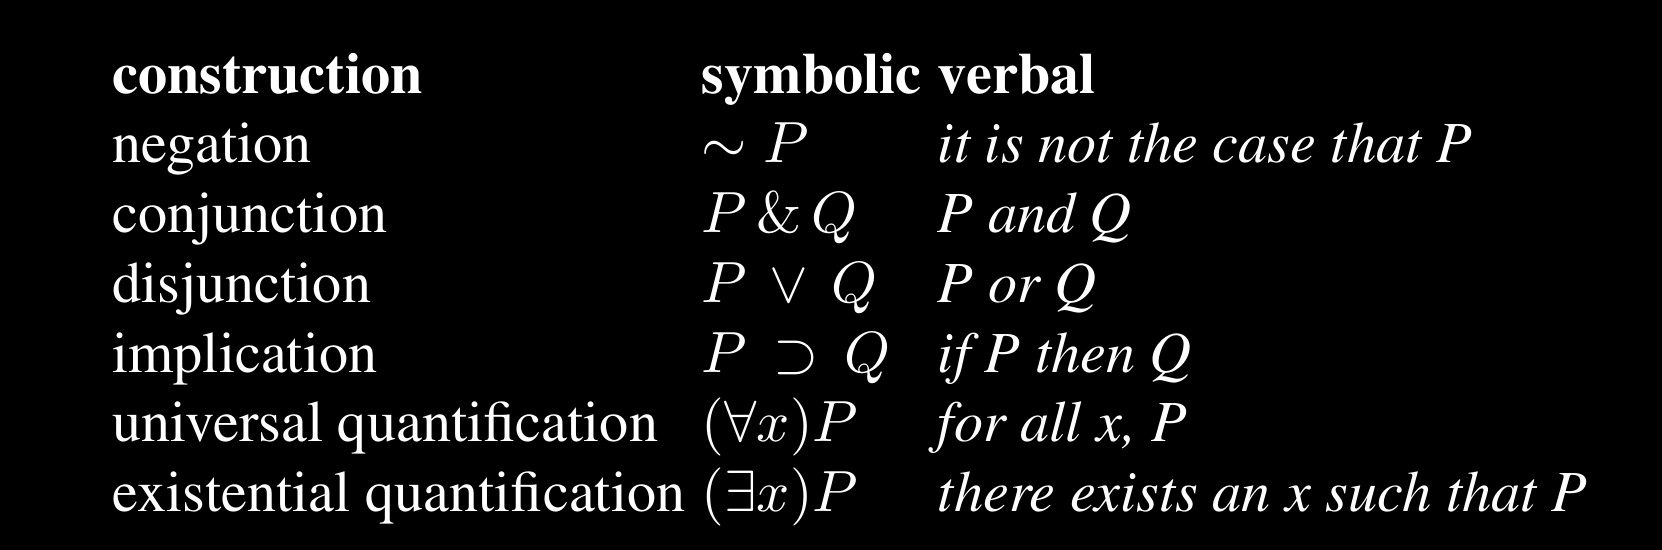
\includegraphics[width= \paperwidth]{core.png}
\end{figure}

\end{frame}

\begin{frame}

\begin{block}{Extended}
\begin{itemize}
\item much more expressive
\item semantically adequate
\item ``every natural number is even or odd"
\item increases both number of categories and functions
\item also need for more complicated linearization categories
\item complex PGF backend to keep this syntactically complete
\item questions about scalability
\end{itemize}

\end{block}

\end{frame}

\begin{frame}
\frametitle{Extended Syntax}

\begin{figure}
\hspace*{-3mm}%
   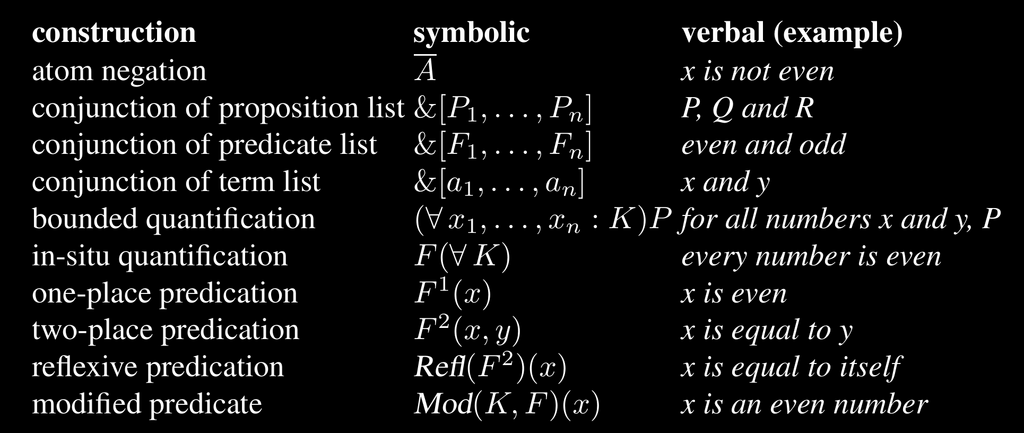
\includegraphics[width= \paperwidth]{e.png}
\end{figure}
\end{frame}
% ``every number is even or odd" (more concise, future research topic)


\begin{frame}
\frametitle{Translation}
$\llbracket - \rrbracket : Extended \to Core$

\begin{itemize}
% think of coq tactics evaluating to gallina terms
\item relatively simple (in the sense that it should be deterministic)
\item More or less uses the same logical structure from the ``standard view"
\item Core syntax as a model for extended
\end{itemize}

\end{frame}

\begin{frame}

$\llbracket - \rrbracket : Core \to Extended$

\begin{itemize}

\item Flattening a list \\
  $x\ and\ y\ and\ z\ \mapsto x,\ y\ and\ z$
\item Aggregation \\
  $x\ is\ even\ or\ x\ is\ odd\ \mapsto x\ is\ even\ or\ odd$
\item In-situ quantification \\
  $\forall\ n\ \in Nat,\ x\ is\ even\ or\ x\ is\ odd \mapsto every\ Nat\ is\ even\ or \odd$
\item Negation \\
  $it\ is\ not\ that\ case\ that\ x\ is\ even\ \mapsto \x is\ not\ even$
\item Reflexivitazion \\
  $x\ is\ equal\ to\ x\ \mapsto x\ is\ equal\ to\ itself$
\item Modification \\
  $x\ is\ a\ number\ and\ x\ is\ even\ \mapsto x\ is\ an\ even\ number$
\end{itemize}
\end{frame}


\subsection{Hott '14}

\begin{frame}
\frametitle{Ranta's (unpublished) talk at Stockholm Math Seminar}
\begin{itemize}
\item Case study for text of \emph{real} mathematics writing
\item Purely GF translation
\item Complex abstract structure including latex, metadocument structure, etc.
\item Homotopy Type Theory (HoTT) specific lexicon
\item Includes proofs, but AST not similar to PL
\item Includes both expressions and propositions (breaks curry howard)
\item Semantically Adequate but syntactically incomplete
\end{itemize}
\end{frame}


\begin{frame}
\frametitle{HoTT Grammar Modules}

\begin{figure}
\hspace*{-3mm}%
   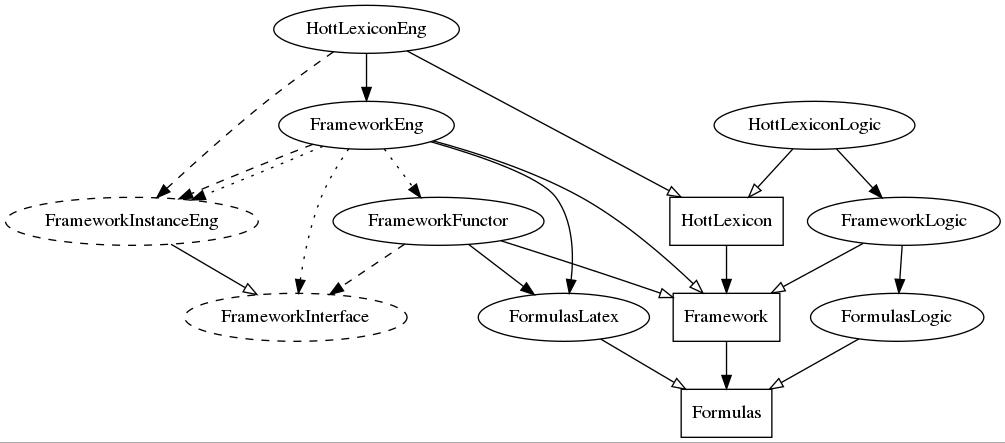
\includegraphics[width= \paperwidth]{testdep3.jpg}
\end{figure}
\end{frame}

\begin{frame}[fragile]
\frametitle{Framework.gf}
\begin{verbatim}
cat
  Paragraph ; -- definition, theorem, etc
  Definition ; -- definition of a new concept
  Assumption ; -- assumption in a proof -- let ...
  [Assumption]{1} ;  -- list of assumptions in one sentence
  Conclusion ; -- conclusion in a proof -- thus P
  Prop ; -- proposition,sentence or formula, A is contractible
  Sort ; -- set, type, etc corresponding to a common noun
  Ind ; -- individual element corresponding to a singular term
  Fun ; -- function with individual value
  Pred ; -- predicate: function with proposition value
  [Ind] ; -- list of individual expressions -- 1, 2 and 3
  UnivPhrase ; -- universal noun phrase -- for all x,y : A
  ConclusionPhrase ; -- conclusion word -- hence
  Label ; -- name/number of definition, theorem, etc
  Title ; -- title for theorem, definition, etc
\end{verbatim}
\end{frame}
\begin{frame}[fragile]

\frametitle{Formulas.gf}
\begin{verbatim}
cat
  Exp ;          -- formal expression             
                 -- x + y = z
  Var ;          -- variable
                 -- x
  [Var]{1} ;     -- list of variables             
                 -- x, y, z
  [Exp]{1} ;     -- list of expressions           
                 -- 1_{A}, A
  Format ;       -- line other than content       
                 -- \begin{document}
  MathEnv ;      -- math environment              
                 -- $ ... $
\end{verbatim}
\end{frame}

\begin{frame}[fragile]
\frametitle{Comparative Syntax}

\begin{itemize}
\item We work with the definition of contractability, the notion that a type (or space) is
actually a point, i.e. up to equality, there is only object. 
\item We show the rendered latex, a pidgin agda syntax (after some concrete
  modifications), and the Agda code
\end{itemize}\\~\\

\textbf{Definition}:
A type $A$ is contractible, if there is $a : A$, called the center of contraction, such that for all $x : A$, $\equalH {a}{x}$.

\\~\\
\begin{figure}
\begin{verbatim}
isContr ( A : Set ) : Set = 
  ( a : A ) ( * ) ( ( x : A ) -> Id ( a ) ( x ) )
\end{verbatim}
\end{figure}


\begin{code}[hide]%
\>[0]\AgdaSymbol{\{-\#}\AgdaSpace{}%
\AgdaKeyword{OPTIONS}\AgdaSpace{}%
\AgdaPragma{--omega-in-omega}\AgdaSpace{}%
\AgdaPragma{--type-in-type}\AgdaSpace{}%
\AgdaSymbol{\#-\}}\<%
\\
%
\\[\AgdaEmptyExtraSkip]%
\>[0]\AgdaKeyword{module}\AgdaSpace{}%
\AgdaModule{contr}\AgdaSpace{}%
\AgdaKeyword{where}\<%
\\
%
\\[\AgdaEmptyExtraSkip]%
\>[0]\AgdaKeyword{open}\AgdaSpace{}%
\AgdaKeyword{import}\AgdaSpace{}%
\AgdaModule{Agda.Builtin.Sigma}\AgdaSpace{}%
\AgdaKeyword{public}\<%
\\
%
\\[\AgdaEmptyExtraSkip]%
\>[0]\AgdaKeyword{variable}\<%
\\
\>[0][@{}l@{\AgdaIndent{0}}]%
\>[2]\AgdaGeneralizable{A}\AgdaSpace{}%
\AgdaGeneralizable{B}\AgdaSpace{}%
\AgdaSymbol{:}\AgdaSpace{}%
\AgdaPrimitive{Set}\<%
\\
%
\\[\AgdaEmptyExtraSkip]%
\>[0]\AgdaKeyword{data}\AgdaSpace{}%
\AgdaOperator{\AgdaDatatype{\AgdaUnderscore{}≡\AgdaUnderscore{}}}\AgdaSpace{}%
\AgdaSymbol{\{}\AgdaBound{A}\AgdaSpace{}%
\AgdaSymbol{:}\AgdaSpace{}%
\AgdaPrimitive{Set}\AgdaSymbol{\}}\AgdaSpace{}%
\AgdaSymbol{(}\AgdaBound{a}\AgdaSpace{}%
\AgdaSymbol{:}\AgdaSpace{}%
\AgdaBound{A}\AgdaSymbol{)}\AgdaSpace{}%
\AgdaSymbol{:}\AgdaSpace{}%
\AgdaBound{A}\AgdaSpace{}%
\AgdaSymbol{→}\AgdaSpace{}%
\AgdaPrimitive{Set}\AgdaSpace{}%
\AgdaKeyword{where}\<%
\\
\>[0][@{}l@{\AgdaIndent{0}}]%
\>[2]\AgdaInductiveConstructor{r}\AgdaSpace{}%
\AgdaSymbol{:}\AgdaSpace{}%
\AgdaBound{a}\AgdaSpace{}%
\AgdaOperator{\AgdaDatatype{≡}}\AgdaSpace{}%
\AgdaBound{a}\<%
\\
%
\\[\AgdaEmptyExtraSkip]%
\>[0]\AgdaKeyword{infix}\AgdaSpace{}%
\AgdaNumber{20}\AgdaSpace{}%
\AgdaOperator{\AgdaDatatype{\AgdaUnderscore{}≡\AgdaUnderscore{}}}\<%
\\
%
\\[\AgdaEmptyExtraSkip]%
\>[0]\AgdaFunction{id}\AgdaSpace{}%
\AgdaSymbol{:}\AgdaSpace{}%
\AgdaGeneralizable{A}\AgdaSpace{}%
\AgdaSymbol{→}\AgdaSpace{}%
\AgdaGeneralizable{A}\<%
\\
\>[0]\AgdaFunction{id}\AgdaSpace{}%
\AgdaSymbol{=}\AgdaSpace{}%
\AgdaSymbol{λ}\AgdaSpace{}%
\AgdaBound{z}\AgdaSpace{}%
\AgdaSymbol{→}\AgdaSpace{}%
\AgdaBound{z}\<%
\\
%
\\[\AgdaEmptyExtraSkip]%
\>[0]\<%
\end{code}

\begin{code}%
\>[0]\<%
\\
\>[0]\AgdaFunction{isContr}\AgdaSpace{}%
\AgdaSymbol{:}\AgdaSpace{}%
\AgdaSymbol{(}\AgdaBound{A}\AgdaSpace{}%
\AgdaSymbol{:}\AgdaSpace{}%
\AgdaPrimitive{Set}\AgdaSymbol{)}\AgdaSpace{}%
\AgdaSymbol{→}\AgdaSpace{}%
\AgdaPrimitive{Set}\<%
\\
\>[0]\AgdaFunction{isContr}\AgdaSpace{}%
\AgdaBound{A}\AgdaSpace{}%
\AgdaSymbol{=}%
\>[13]\AgdaRecord{Σ}\AgdaSpace{}%
\AgdaBound{A}\AgdaSpace{}%
\AgdaSymbol{λ}\AgdaSpace{}%
\AgdaBound{a}\AgdaSpace{}%
\AgdaSymbol{→}\AgdaSpace{}%
\AgdaSymbol{(}\AgdaBound{x}\AgdaSpace{}%
\AgdaSymbol{:}\AgdaSpace{}%
\AgdaBound{A}\AgdaSymbol{)}\AgdaSpace{}%
\AgdaSymbol{→}\AgdaSpace{}%
\AgdaSymbol{(}\AgdaBound{a}\AgdaSpace{}%
\AgdaOperator{\AgdaDatatype{≡}}\AgdaSpace{}%
\AgdaBound{x}\AgdaSymbol{)}\<%
\\
%
\\[\AgdaEmptyExtraSkip]%
\>[0]\<%
\end{code}


\end{frame}

\begin{frame}[fragile]

\begin{itemize}
\item We also show that a notion of a map being an equivalence, that of the
  every element in the codomain having a contractible image (think bijection) 
\item notice the error in the Pidgin case
\end{itemize}

\\~\\

 \textbf{Definition}:
 A map $f : \arrowH {A}{B}$ is an equivalence, if for all $y : B$, its fiber, $\comprehensionH {x}{A}{\equalH {\appH {f}{x}}{y}}$, is contractible.
 We write $\equivalenceH {A}{B}$, if there is an equivalence $\arrowH {A}{B}$.

\\~\\

\begin{figure}
\begin{verbatim}
Equivalence ( f : A -> B ) : Set = 
  ( y : B ) -> ( isContr ( fiber it ) ) ; ; ; 
  fiber it : Set = ( x : A ) ( * ) ( Id ( f ( x ) ) ( y ) )
\end{verbatim}
\end{figure}


\begin{code}[hide]%
\>[0]\AgdaSymbol{\{-\#}\AgdaSpace{}%
\AgdaKeyword{OPTIONS}\AgdaSpace{}%
\AgdaPragma{--omega-in-omega}\AgdaSpace{}%
\AgdaPragma{--type-in-type}\AgdaSpace{}%
\AgdaSymbol{\#-\}}\<%
\\
%
\\[\AgdaEmptyExtraSkip]%
\>[0]\AgdaKeyword{module}\AgdaSpace{}%
\AgdaModule{equiv}\AgdaSpace{}%
\AgdaKeyword{where}\<%
\\
%
\\[\AgdaEmptyExtraSkip]%
\>[0]\AgdaKeyword{open}\AgdaSpace{}%
\AgdaKeyword{import}\AgdaSpace{}%
\AgdaModule{Agda.Builtin.Sigma}\AgdaSpace{}%
\AgdaKeyword{public}\<%
\\
%
\\[\AgdaEmptyExtraSkip]%
\>[0]\AgdaKeyword{variable}\<%
\\
\>[0][@{}l@{\AgdaIndent{0}}]%
\>[2]\AgdaGeneralizable{A}\AgdaSpace{}%
\AgdaGeneralizable{B}\AgdaSpace{}%
\AgdaSymbol{:}\AgdaSpace{}%
\AgdaPrimitive{Set}\<%
\\
%
\\[\AgdaEmptyExtraSkip]%
\>[0]\AgdaKeyword{data}\AgdaSpace{}%
\AgdaOperator{\AgdaDatatype{\AgdaUnderscore{}≡\AgdaUnderscore{}}}\AgdaSpace{}%
\AgdaSymbol{\{}\AgdaBound{A}\AgdaSpace{}%
\AgdaSymbol{:}\AgdaSpace{}%
\AgdaPrimitive{Set}\AgdaSymbol{\}}\AgdaSpace{}%
\AgdaSymbol{(}\AgdaBound{a}\AgdaSpace{}%
\AgdaSymbol{:}\AgdaSpace{}%
\AgdaBound{A}\AgdaSymbol{)}\AgdaSpace{}%
\AgdaSymbol{:}\AgdaSpace{}%
\AgdaBound{A}\AgdaSpace{}%
\AgdaSymbol{→}\AgdaSpace{}%
\AgdaPrimitive{Set}\AgdaSpace{}%
\AgdaKeyword{where}\<%
\\
\>[0][@{}l@{\AgdaIndent{0}}]%
\>[2]\AgdaInductiveConstructor{r}\AgdaSpace{}%
\AgdaSymbol{:}\AgdaSpace{}%
\AgdaBound{a}\AgdaSpace{}%
\AgdaOperator{\AgdaDatatype{≡}}\AgdaSpace{}%
\AgdaBound{a}\<%
\\
%
\\[\AgdaEmptyExtraSkip]%
\>[0]\AgdaKeyword{infix}\AgdaSpace{}%
\AgdaNumber{20}\AgdaSpace{}%
\AgdaOperator{\AgdaDatatype{\AgdaUnderscore{}≡\AgdaUnderscore{}}}\<%
\\
%
\\[\AgdaEmptyExtraSkip]%
\>[0]\AgdaFunction{id}\AgdaSpace{}%
\AgdaSymbol{:}\AgdaSpace{}%
\AgdaGeneralizable{A}\AgdaSpace{}%
\AgdaSymbol{→}\AgdaSpace{}%
\AgdaGeneralizable{A}\<%
\\
\>[0]\AgdaFunction{id}\AgdaSpace{}%
\AgdaSymbol{=}\AgdaSpace{}%
\AgdaSymbol{λ}\AgdaSpace{}%
\AgdaBound{z}\AgdaSpace{}%
\AgdaSymbol{→}\AgdaSpace{}%
\AgdaBound{z}\<%
\\
%
\\[\AgdaEmptyExtraSkip]%
\>[0]\AgdaFunction{isContr}\AgdaSpace{}%
\AgdaSymbol{:}\AgdaSpace{}%
\AgdaSymbol{(}\AgdaBound{A}\AgdaSpace{}%
\AgdaSymbol{:}\AgdaSpace{}%
\AgdaPrimitive{Set}\AgdaSymbol{)}\AgdaSpace{}%
\AgdaSymbol{→}\AgdaSpace{}%
\AgdaPrimitive{Set}\<%
\\
\>[0]\AgdaFunction{isContr}\AgdaSpace{}%
\AgdaBound{A}\AgdaSpace{}%
\AgdaSymbol{=}%
\>[13]\AgdaRecord{Σ}\AgdaSpace{}%
\AgdaBound{A}\AgdaSpace{}%
\AgdaSymbol{λ}\AgdaSpace{}%
\AgdaBound{a}\AgdaSpace{}%
\AgdaSymbol{→}\AgdaSpace{}%
\AgdaSymbol{(}\AgdaBound{x}\AgdaSpace{}%
\AgdaSymbol{:}\AgdaSpace{}%
\AgdaBound{A}\AgdaSymbol{)}\AgdaSpace{}%
\AgdaSymbol{→}\AgdaSpace{}%
\AgdaSymbol{(}\AgdaBound{a}\AgdaSpace{}%
\AgdaOperator{\AgdaDatatype{≡}}\AgdaSpace{}%
\AgdaBound{x}\AgdaSymbol{)}\<%
\\
\>[0]\<%
\end{code}

\begin{code}%
\>[0]\<%
\\
%
\\[\AgdaEmptyExtraSkip]%
\>[0]\AgdaFunction{Equivalence}\AgdaSpace{}%
\AgdaSymbol{:}\AgdaSpace{}%
\AgdaSymbol{(}\AgdaBound{A}\AgdaSpace{}%
\AgdaBound{B}\AgdaSpace{}%
\AgdaSymbol{:}\AgdaSpace{}%
\AgdaPrimitive{Set}\AgdaSymbol{)}\AgdaSpace{}%
\AgdaSymbol{→}\AgdaSpace{}%
\AgdaSymbol{(}\AgdaBound{f}\AgdaSpace{}%
\AgdaSymbol{:}\AgdaSpace{}%
\AgdaBound{A}\AgdaSpace{}%
\AgdaSymbol{→}\AgdaSpace{}%
\AgdaBound{B}\AgdaSymbol{)}\AgdaSpace{}%
\AgdaSymbol{→}\AgdaSpace{}%
\AgdaPrimitive{Set}\<%
\\
\>[0]\AgdaFunction{Equivalence}\AgdaSpace{}%
\AgdaBound{A}\AgdaSpace{}%
\AgdaBound{B}\AgdaSpace{}%
\AgdaBound{f}\AgdaSpace{}%
\AgdaSymbol{=}\AgdaSpace{}%
\AgdaSymbol{∀}\AgdaSpace{}%
\AgdaSymbol{(}\AgdaBound{y}\AgdaSpace{}%
\AgdaSymbol{:}\AgdaSpace{}%
\AgdaBound{B}\AgdaSymbol{)}\AgdaSpace{}%
\AgdaSymbol{→}\AgdaSpace{}%
\AgdaFunction{isContr}\AgdaSpace{}%
\AgdaSymbol{(}\AgdaFunction{fiber'}\AgdaSpace{}%
\AgdaBound{y}\AgdaSymbol{)}\<%
\\
\>[0][@{}l@{\AgdaIndent{0}}]%
\>[2]\AgdaKeyword{where}\<%
\\
\>[2][@{}l@{\AgdaIndent{0}}]%
\>[4]\AgdaFunction{fiber'}\AgdaSpace{}%
\AgdaSymbol{:}\AgdaSpace{}%
\AgdaSymbol{(}\AgdaBound{y}\AgdaSpace{}%
\AgdaSymbol{:}\AgdaSpace{}%
\AgdaBound{B}\AgdaSymbol{)}\AgdaSpace{}%
\AgdaSymbol{→}\AgdaSpace{}%
\AgdaPrimitive{Set}\<%
\\
%
\>[4]\AgdaFunction{fiber'}\AgdaSpace{}%
\AgdaBound{y}\AgdaSpace{}%
\AgdaSymbol{=}\AgdaSpace{}%
\AgdaRecord{Σ}\AgdaSpace{}%
\AgdaBound{A}\AgdaSpace{}%
\AgdaSymbol{(λ}\AgdaSpace{}%
\AgdaBound{x}\AgdaSpace{}%
\AgdaSymbol{→}\AgdaSpace{}%
\AgdaBound{y}\AgdaSpace{}%
\AgdaOperator{\AgdaDatatype{≡}}\AgdaSpace{}%
\AgdaBound{f}\AgdaSpace{}%
\AgdaBound{x}\AgdaSymbol{)}\<%
\\
\>[0]\<%
\end{code}


\end{frame}

\begin{frame}

\frametitle{This project}

\end{frame}

\begin{frame}
\frametitle{Future Work}

Convert mathematicians.
More interaction between PL communities - Lean, Agda, Coq , {Prl} -
These languages each represent a  huge field of interrelated and independent research.

Linguistic analysis.  Gangaselem's work is both practical and philosophical,
both directions need a lot more research

A mathematician objected that it can't be difficult to prove a 2 is prime in
Agda. This is because they in some sense are mixing definitional and
propositional equality.

Prop equality <-> isomorphism via univalence, but even moreso after cubical

HITs <-> new proofs, new discoveries more akin to semantic feeling

A FORMAL SYSTEM FOR EUCLID’S ELEMENTS
https://www.cambridge.org/core/journals/review-of-symbolic-logic/article/abs/formal-system-for-euclids-elements/07CA7E5F8E1C5C2EB632E1005CBE7BEF

Different intersecting ideas of models, syntax vs semantic

Krasimir : bigger grammar, begins resembling RGL
(but we also need to
investigate where compile time optimizations are necessary for this)
We need an RGL to take care of things that satisfy both the Computer Scientists,
Logicians, and Mathematicians

TODO:


- pattern matching (Agda) perhaps ad-hoc, post processing necessary
- GF latex RGL (at least for some of it)
- domain corpus for comparison of concrete syntax's
- testing suite, framework, and methodology (specifically, for formal language CNLs)
- some work on GF itself, to allow for user defined categories (like Int and
String for variables)
- interface with the Agda community.  Alfa and GF grew together, and its a shame
they parted ways.
- possible investigation of metaprogramming in GF (this may hit the parser
complexity bottleneck)
- Mathematical Theory of GF will us to understand GF more formally, i.e. prove
theorems about the adjunction between Concrete and Abstract
- inference to determine type signature arities (Abstract seems the way to go,
although with hidden variables this becomes an exponential problem in terms of
the type signatures

Diagram about what is a model and what is syntax in GF

While Machine learning enthusisasts (Szegedy, ...) think that Proving,
Translating, etc are feasible, it is certainly our belief that this is very
wishful thinking.  If this work has taught me anything, its that the
mathematical way of thinking, presenting, and communicating is complex and nuanced in ways
are digital technologies aren't yet able to do much with (even with lots of
human labor)

\end{frame}


\end{document}
